%\documentclass[11pt, oneside]{article}  

%\usepackage{style-3yp} %this is the .sty file
%\usepackage{pdflscape}
\lfoot{Enzia Schnyder} %your name in the footer

%\usepackage{float}
%\usepackage{longtable}
%table
%\usepackage{array}
%\newcolumntype{L}{>{\centering\arraybackslash}m{2.5cm}}
%\newcolumntype{J}{>{\centering\arraybackslash}m{4.1cm}}
%\newcolumntype{M}{>{\centering\arraybackslash}m{5cm}}
%\newcolumntype{N}{>{\centering\arraybackslash}m{3.5cm}}
%\usepackage{multirow}

%\usepackage{gensymb} %degrees symbol
%\usepackage [version=4] {mhchem}


%\begin{document}

\part{Precracker}

\section{Introduction}
As examined in this section of the report, ammonia presents many difficulties as a fuel. This means that it must be cracked before passing through the turbine. A suitable ratio was found for the mixture... %finish this

\section{Limitations of Ammonia as a Fuel \cite{verkamp}}
Ammonia provides many challenges as a combustible fuel. Its high ignition energy, high heat of vapourisation and low lower calorific value (LCV) mean that a lot of energy must be put into combustion. Additionally, it also has narrow flammability limits, meaning that it will burn only in a narrow range of equivalence ratios.  Different methods to mitigate this that were considered were:
\begin {enumerate}
\item Mixing hydrocarbons into the ammonia. - This would improve combustion properties but at the cost of a high negative environmental impact due to the carbon emissions and the impact of extracting and transporting natural gas to the plant. 
\item Burn a mixture of ammonia and hydrogen. - The burning properties of hydrogen are much better than ammonia. A precracker can be used to partially dissociate the ammonia into hydrogen and nitrogen so that a mixture of the three gases is burned in the combustion chamber. As Verkamp et.al. showed, a ratio of 28\% hydrogen leads to combustion properties comparable to that of hydrocarbons. 
\item Gas turbine modifications. - A standard gas turbine can be modified to burn ammonia, which would include using a higher input ignition energy and greater area to accommodate for decreased air flow rate due to the lower flame stability of ammonia. However, this would be very expensive in both capital and operating costs.
\end {enumerate}

It was decided to use methods 2 and 3 together to improve ammonia combustion. A precracker will be used to partially dissociate the ammonia coming from storage, which will be burnt in the combustion chamber with air and the waste oxygen from the electrolyser.

\subsection{Dissociation Ratio - P36}
To find the appropriate dissociation ratio, the properties of ammonia and hydrogen were compared with conventional fuels diesel and gasoline as shown in table \ref{tab:burningproperties}.

\begin{table} [h]
\begin{center}
\caption{The burning properties of ammonia, hydrogen, diesel and gasoline \cite{garabedian}}\label{tab:burningproperties}
\begin{tabular}{ |c|c|L|L|L|L| }
 \hline
  Fuel & LCV (MJ/kg) \cite{website:spg} & Ignition Energy (mJ) & Stoichiometric AFR by mass & Autoignition Temperature (\degree F) & Flame Speed (cm/s) \\ 
 \hline
  $NH_3$ & 18.6 & 9.0 & 0.1653 & 1200 & 33 \\ 
 \hline
$H_2$ & 120.1 & 0.18 & 0.0292 & 1170 & 300\\ 
 \hline
Diesel & 42.8 & 0.3 & 0.068 & 500 & 100\\
 \hline
 Gasoline & 42.5 & 0.3 & 0.068 & 800 & 100\\
 \hline
\end{tabular}
\end{center} 
\end{table}


A tradeoff must be found between optimising burning properties and having too much hydrogen, which will lead to an unstable, rapid burning and high combustion temperatures. 

  \begin{figure} [h]
\centering
\begin{subfigure}{.5\textwidth}
  \centering
  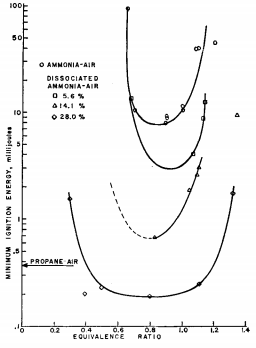
\includegraphics[width=0.9\linewidth]{./pictures/ignitionenergyNH3.png}
  \label{fig:mixproperties1}
\end{subfigure}%
\begin{subfigure}{.5\textwidth}
  \centering
  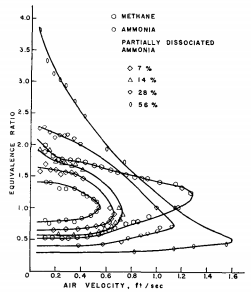
\includegraphics[width=0.9\linewidth]{./pictures/flamestabilityNH3.png}
  \label{fig:sub2}
\end{subfigure}
\caption{(a) The ignition energy and (b) flame-stability properties of methane-air, ammonia-air and partially dissociated ammonia-air \cite{verkamp}}
\label{fig:mixproperties2}
\end{figure} %better quality pictures

The figure \ref{fig:mixproperties2} suggests that 28\% dissociation still had a minimum ignition energy higher than that of propane-air (8mJ compared to 0.37mJ at a similar equivalence ratio), which suggests a higher dissociation is required. Li et. al. \cite{junli} also showed that 54.5\% dissociation had a similar burning velocity to methane. We want the mixture to behave similarly to natural gas, which is composed of methane (93.9\%), ethane (4.2\%) and propane (0.3\%), so that no modifications need to be made to the turbine. Therefore a dissociation of 38\% will be used with dissociation reaction:

\begin{equation}
\ce{NH_3 -> 0.62 NH_3 + 0.19 N_2 + 0.57 H_2}
\end{equation}

Assuming that dry air is made of 79\% $N_2^*$ and 21\% $O_2$ where $N_2^*$ is used to represents all components of air other than oxygen the combustion reaction for one mole of pre-cracked ammonia is:
\begin{equation}
\ce{(0.62 NH_3 + 0.19 N_2 + 0.57 H_2) + 0.75(O_2 + 3.76 N_2^*) ->1.5H_2O + 0.5N_2 + 2.82N_2^*}
\end{equation}

\subsection {Mixture Properties}
Properties of the new mixture are summarised in table \ref{tab:mixproperties}. The molar mass and lower calorific value were calculated using a weighted sum of the relevant mixture components i.e.
\begin{equation}
M_{r, mix} = \sum_{i=1}^{N} x_i M_{r,i}
\end{equation}
Where $M_{r, i}$ is the molar mass and $x_i$ is the mole fraction of the i-th component of the mixture. 

Lower flammability limits (LFL) and upper flammability limits (UFL) are the limits by volume percentage where combustion can occur. The flammability limits of the mixture were calculated using Le Chatelier's mixing rule \cite{chat}: 
\begin{equation}
FL_{mix} = \frac{1}{\sum_{i=1}^{N} \frac{x_i}{FL_i}}
\end{equation}
Where $FL_{i}$ is the upper or lower flammability limit of the i-th component of the mixture. The volume percentage of $H_2/NH_3$ at stoichiometric combustion is 24\%, which falls comfortably in the flammability limits.

\begin{table} [h]
\begin{center}
\caption{Properties of the ammonia-air mixture. Due to its inert nature, the nitrogen formed in precracking ammonia were excluded in the calculations for flammability limits and calorific value. \cite{FL}} \label{tab:mixproperties}
\begin{tabular}{ |c|c|c|c|c|c| }
 \hline
& Mr (a.m.u) & LCV (MJ/kg) \cite{website:spg}& LCV (MJ/kmol) & LFL & UFL\\ 
 \hline
  $H_2$ & 2.02 & 120.1 & 242.6 & 4.0 & 75.0\\ 
 \hline
$NH_3$ & 17.03 & 18.6 & 316.8 & 15.0 & 28.0\\ 
 \hline
$H_2/NH_3$ mixture & 10 & 28.6 & 334.7 & 6.47 & 40\\
 \hline
\end{tabular}
\end{center} 
\end{table}

\bibliography{./turbine/precracker}
\bibliographystyle{unsrt}
%\end{document}